\chapter{Implementace}

V této části bakalářské práce se zaměříme na praktickou implementaci evolučních algoritmů. Kromě toho je nutné ale i implementovat fyzikální prostředí, podobné tomu jako je ve hře polybridge. V první řadě se zaměříme aby se naše simulace co nejvěrněji podobala hře, což umožní použít řešení navrhnuté evolučními algoritmy i ve hře. Nasledně navrhneme několik různých podob evolučního algoritmu pro stavbu mostu a ty mezi sebou porovnáme.


\section{Fyzikální engine}

Jako fyzikální engine pro simulaci jsme zvolili Box2D (citace Box2D). Box2D je open-source fyzikální engine, který poskytuje simulaci pohybu objektů ve 2D prostoru. Je často využíván ve vývoji počítačových her ale také simulací a umožňuje snadné zpracování kolizí, gravitace, tuhosti objektů a dalších fyzikálních jevů. Tento engine byl původně implementován v jazyce C++, avšak díky dostupným knihovnám jej můžeme používat Pythonu, což zvyšuje jeho rychlost a umožňuje nám iterovat přes rozsáhlé množství simulací.

\section{Aproximace hře Poly Bridge}

V naší simulaci jsme implementovali různé aspekty hry pomocí následujících komponent knihovny Box2D:

\begin{itemize}
    \item \textbf{Materiály}: Ty jsou modelovány jako dynamické objekty, pro které používáme \texttt{Box2D.b2DynamicBody}. (odkaz na dokumentaci)
    \item \textbf{Klouby}: Pro spojení různých materiálů jsme využili \texttt{Box2D.b2RevoluteJoint}. (odkaz na dokumentaci)
    \item \textbf{Zátež na prvky}: Abychom zjistili síly působící na jednotlivé elementy v simulaci, používáme metodu \texttt{b2body.GetReactionForce()}, která vrací reakční sílu vzniklou v důsledku interakcí těles. (odkaz na dokumentaci)
\end{itemize}

\subsection{Testy}

Abychom v naší simulaci co nejvěrněji napodobili chování fyzikálních prvků jako ve hře polybridge, zavedli jsme šest různých testů. Tyto testy zkoumají aspekty fyzikální simulace, jako jsou odolnost materiálů v proměnlivých podmínkách, hmotnost materiálů a interakci sil mezi objekty.

Zvolené testy jsou následující:

\begin{enumerate}
    \item \textbf{$2$ vozovky mezi dvěma pevnými body} Očekávaným výsledkem je, že konstrukce praskne pod zatížením samotných vozovek.
    \item \textbf{$6$ dřevěných dílů mezi dvěma pevnými body} Očekáváme, že konstrukce vydrží bez prasknutí.
    \item \textbf{$7$ dřevěných dílů mezi dvěma pevnými body} V tomto testu očekáváme, že konstrukce pod tíhou praskne.
    \item \textbf{Symetrický obrazec z $13.66$ metrů vozovky, zavěšený na jednom kusu vozovky} Testujeme, zda vozovka unese zatížení bez prasknutí.
    \item \textbf{Symetrický obrazec z $14.66$ metrů vozovky, zavěšený na jednom kusu vozovky} V tomto případě testujeme, zda konstrukce nevydrží zatížení a praskne.
    \item \textbf{Komplexní most z vozovek a dřeva, po kterém přejede auto} Cílem tohoto testu je prozkoumat interakci sil mezi různými materiály, kdy očekáváme, že most vydrží přejetí auta.
\end{enumerate}

Vizualizaci testů můžeme vidět na obrázku \ref{impl-fig:1}

\begin{figure}[ht]
    \centering
    \begin{minipage}{0.49\textwidth}
        \centering
        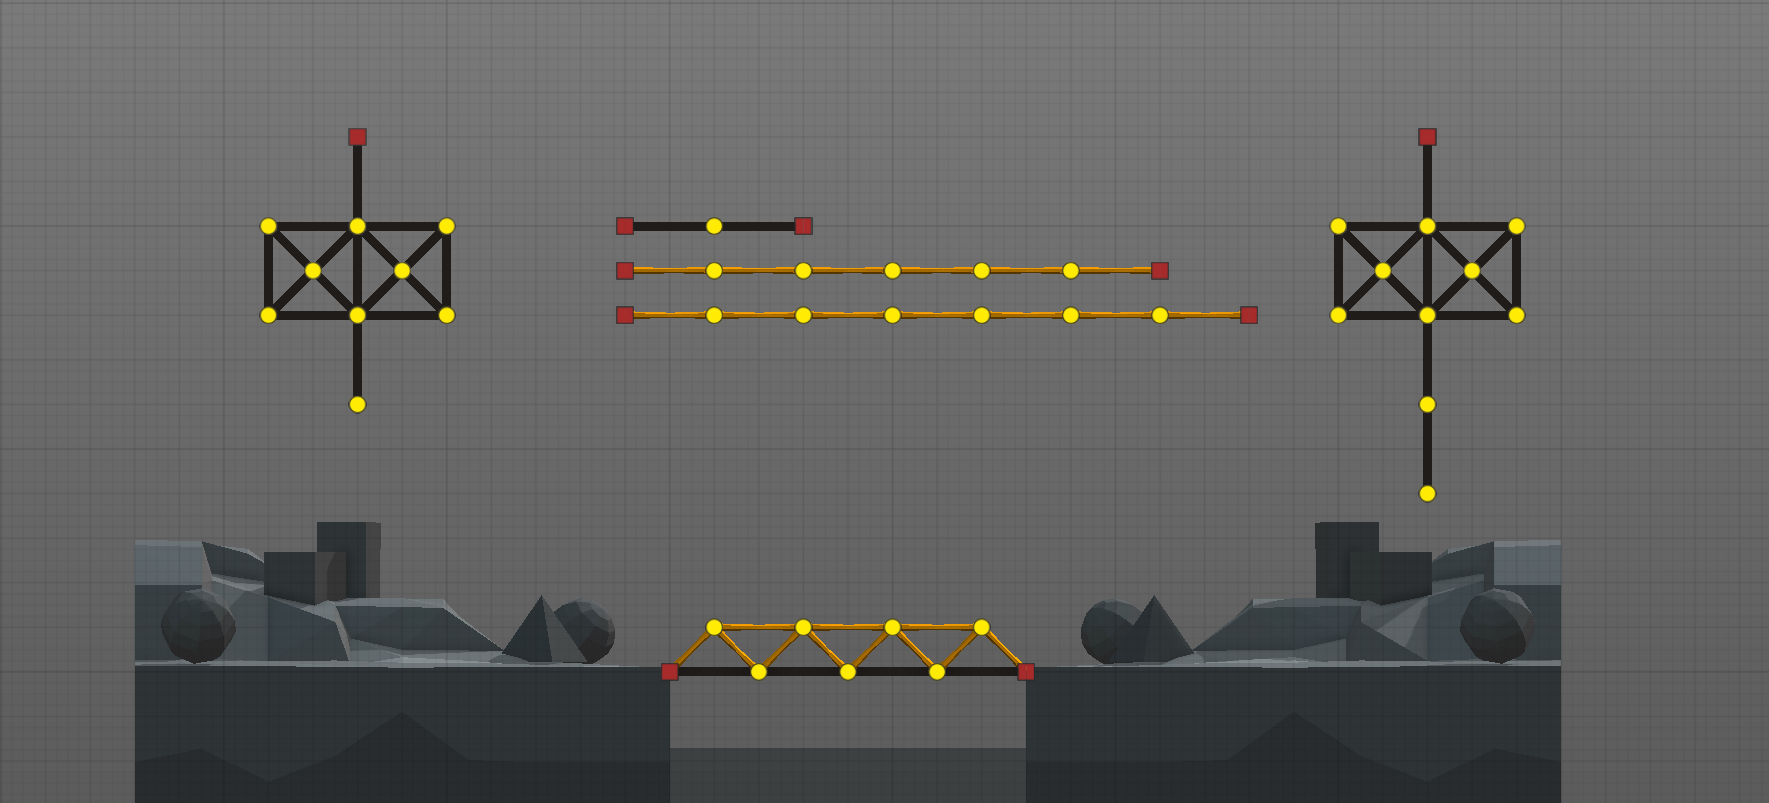
\includegraphics[width=\linewidth]{img/poly_tests.png}
    \end{minipage}\hfill
    \begin{minipage}{0.49\textwidth}
        \centering
        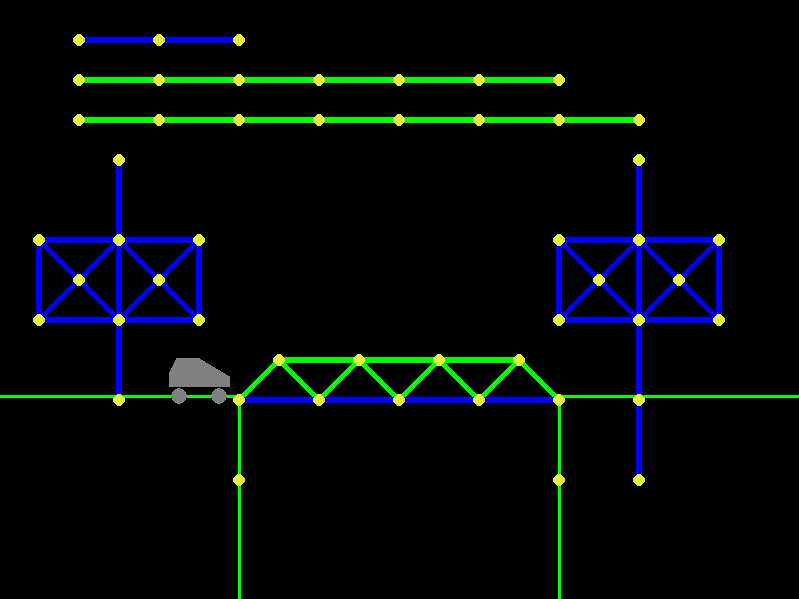
\includegraphics[width=\linewidth]{img/sim_tests.png}
    \end{minipage}
    \caption{Vizualizace testů ve hře polybridge (vlevo) a v simulaci (vpravo)}
    \label{impl-fig:1}
\end{figure}

Naše implementace simulace ma $4$ různé parametry. Těmi jsou \texttt{Box2D.b2Density} hustota materiálů pro dřevo, \texttt{Box2D.b2Density} hustota materiálů pro vozovku, maximální zatížení dřeva a maximální zatížení vozovky. Pro tyto parametry jsme spustili \textit{Random search}(citace random serach) a abychom vybrali ty, které splní nejvíce testů. Bohužel se nám nepodařilo najít takové parametry, abychom splnili všechny. Rozhodli jsme se že $5.$ vyřadíme.

\subsection{Úrovně}

Jako testovací prostředí pro evoluční agloritmus jsme zvolili první $4$ úrovně z původní hry. Více úrovní jsem kvůli jejich komplexitě nezahrnuli.

\begin{figure}[ht]
    \centering
    \begin{minipage}{0.49\textwidth}
        \centering
        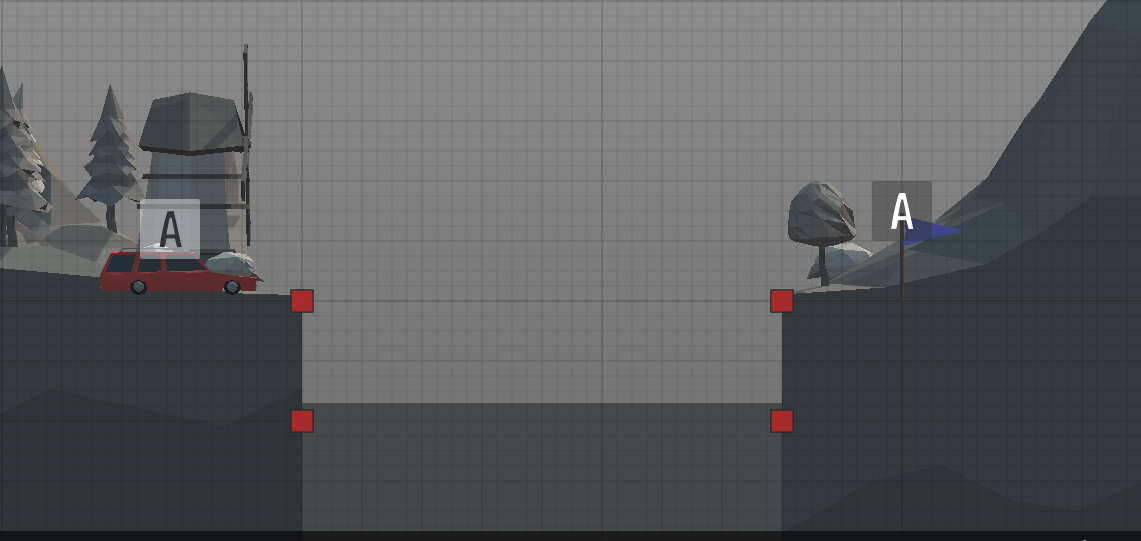
\includegraphics[width=\linewidth]{img/poly_lvl1.png}
    \end{minipage}\hfill
    \begin{minipage}{0.49\textwidth}
        \centering
        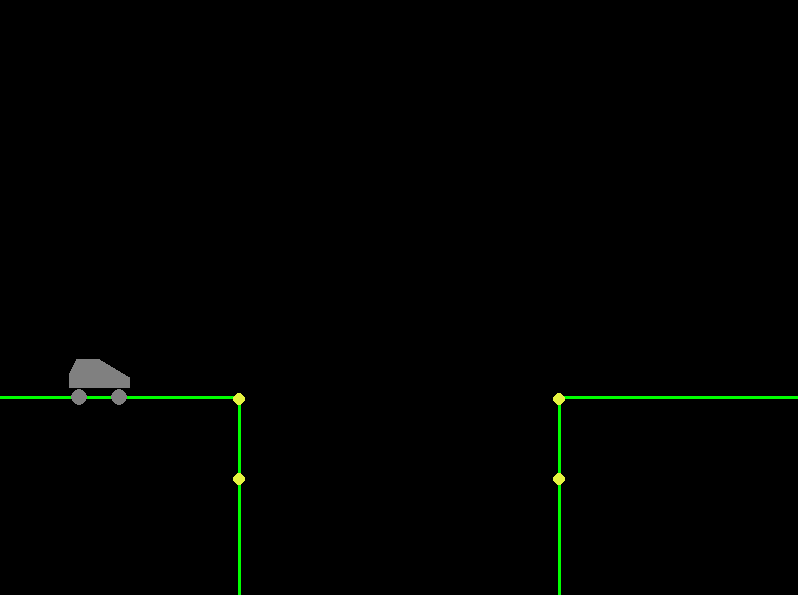
\includegraphics[width=\linewidth]{img/impl_lvl1.png}
    \end{minipage}
    \caption{Vizualizace $1.$ úrovně ve hře polybridge (vlevo) a v simulaci (vpravo)}
    \label{impl-fig:2}
\end{figure}

\begin{figure}[ht]
    \centering
    \begin{minipage}{0.49\textwidth}
        \centering
        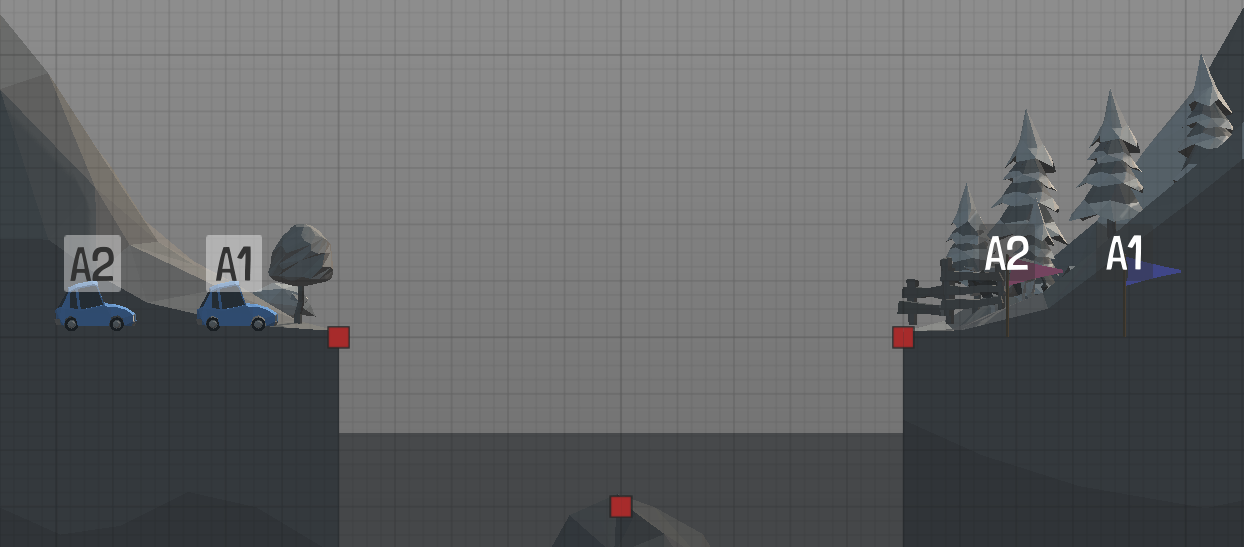
\includegraphics[width=\linewidth]{img/poly_lvl2.png}
    \end{minipage}\hfill
    \begin{minipage}{0.49\textwidth}
        \centering
        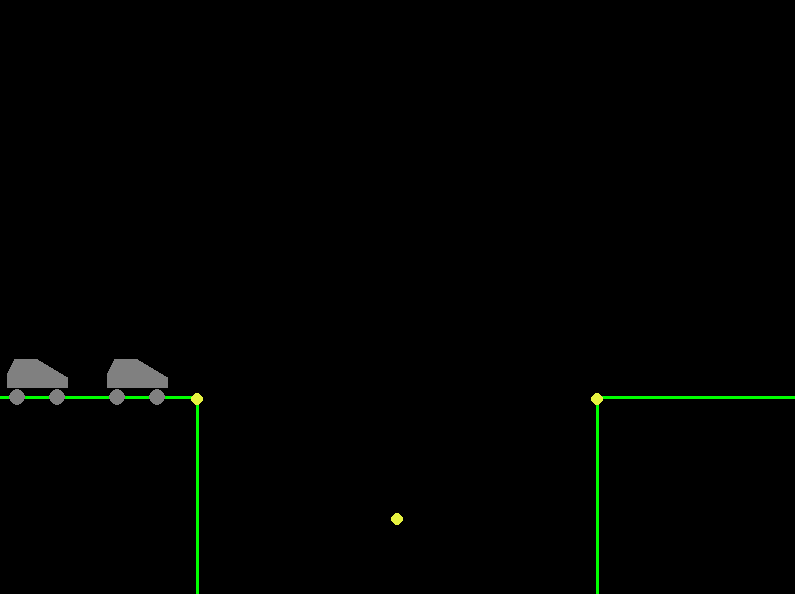
\includegraphics[width=\linewidth]{img/impl_lvl2.png}
    \end{minipage}
    \caption{Vizualizace $2.$ úrovně ve hře polybridge (vlevo) a v simulaci (vpravo)}
    \label{impl-fig:3}
\end{figure}

\begin{figure}[ht]
    \centering
    \begin{minipage}{0.49\textwidth}
        \centering
        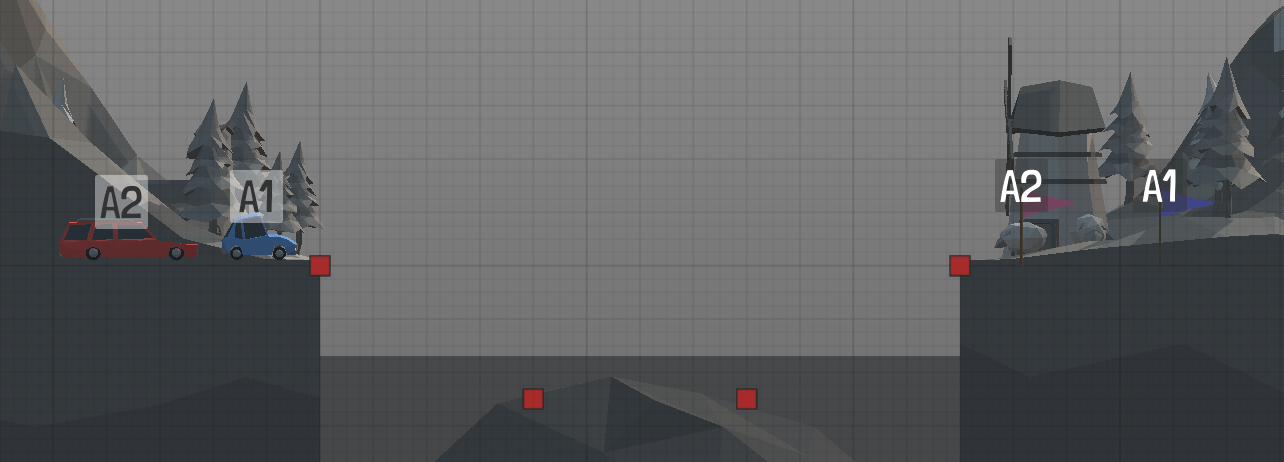
\includegraphics[width=\linewidth]{img/poly_lvl3.png}
    \end{minipage}\hfill
    \begin{minipage}{0.49\textwidth}
        \centering
        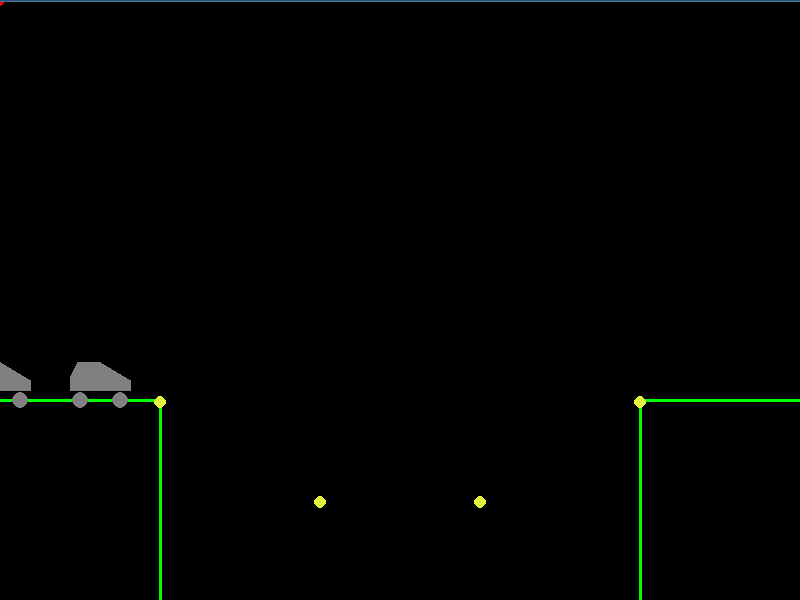
\includegraphics[width=\linewidth]{img/impl_lvl3.png}
    \end{minipage}
    \caption{Vizualizace $3.$ úrovně ve hře polybridge (vlevo) a v simulaci (vpravo)}
    \label{impl-fig:4}
\end{figure}

\begin{figure}[ht]
    \centering
    \begin{minipage}{0.49\textwidth}
        \centering
        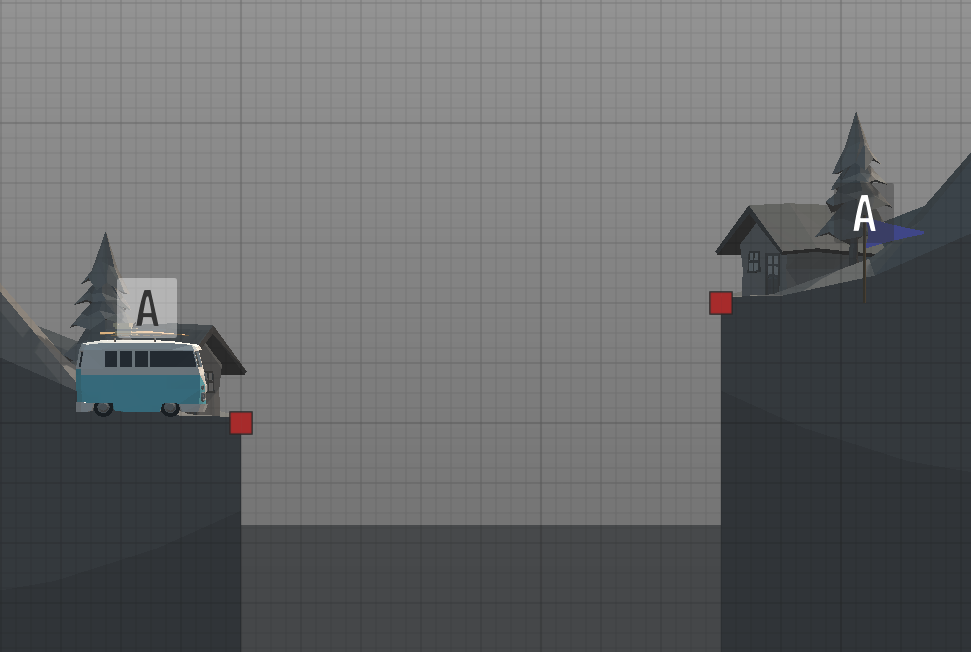
\includegraphics[width=\linewidth]{img/poly_lvl4.png}
    \end{minipage}\hfill
    \begin{minipage}{0.49\textwidth}
        \centering
        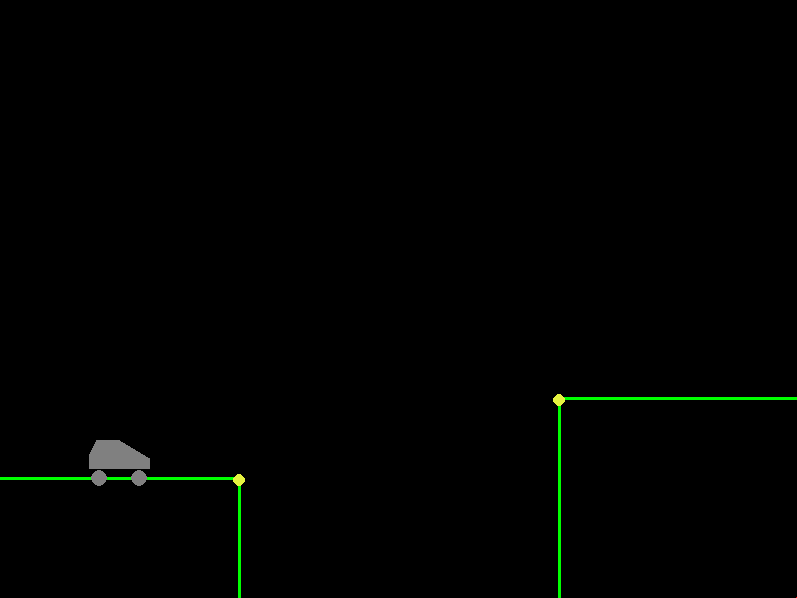
\includegraphics[width=\linewidth]{img/impl_lvl4.png}
    \end{minipage}
    \caption{Vizualizace $4.$ úrovně ve hře polybridge (vlevo) a v simulaci (vpravo)}
    \label{impl-fig:5}
\end{figure}


\section{Aplikace evolučních algoritmů}

V následující sekci ukážem, jak jsem navrhli různé typy genetický operátorů. Budeme používa následující značeni.

\begin{itemize}
    \item $l_{max}$ je maximální délka materiálu
    \item $T$ je množina všech materiálů, které můžeme použít (vozovka, dřevo, nic)
    \item $g$ je gen jedince, nebo také jeden konkrétní most
    \item $d_{min}(g)$ minimální vzdálenost vozidla od urovní definovaného bodu na druhé straně řeky, které se podařilo dosáhnout v simulaci
    \item $cost(g)$ cena mostu $g$
\end{itemize}

Ve všech případech se snažíme optimalizovat dvě hodnoty a to jak daleko naše vozidlo dojelo a cenu mostu. V rámci algoritmu se tedy primárně snažíme maximalozovat $-d_{max}(g)$ a sekundárně $-cost(g)$.

Naše fintess funcke $f$ bude tedy udávaná dvojicí čísel $f(g) = (-d_{min}(g), -cost(g))$

\subsection{Jednoduchý návrh}

Nejednušší návrh danému problému by mohl vypadat následovně. Reprezentace genu je vektor dvojic čísel $c \in \{([0, \dots, x_{max}] \times [0, \dots, y_{max}])\}^n$ kde $x_{max} \in \N$ a $y_{max} \in \N$ je šířka a výška úrovně a vektor $t \in T^n$. Vektor $c$ představuje, serii kliknutí myši na obrazovku a $t$ jaký typ materiálu přidáme.

Jake mutaci jsme zvolili náhodné posunutí pozice kliknutí od $\pm 1$ s pravděpodobností $\frac{1}{n}$ a náhodnout změnu metariálu s pravděpodobností $\frac{1}{n}$.

Jako křížení jsme použili jednobodové křížení vektoru $c$  a $t$ podle stejně zvoleného náhodného bodu. Jako selekci jsme zvolili turnajovou selekci.

Jak můžeme vidět v experimentu (odkaz experiment), algortimu se nedaří stavět příliš kvalitní mosty. Domníváme se, že by tomu tak je z následujících důvodů.

\begin{itemize}
    \item Z principu reprezentace jedince je nepravděpodobné, aby vznikaly krátké hrany, které mohou být klíčové pro kvalitní řešení.
    \item I malá mutace na začátku genu může mít velký vliv na celkovou strukturu mostu.
    \item Křížení v naší reprezentaci nedává smysl.
    \item Fitness funkce nevrací dobrou zpětnou vazbu o kvalitě jedince (viz. obrázek \ref{impl-fig:6})
\end{itemize}

\subsection{Polární kódování}

Kvůli tomu, jak jsme reprezentovali jedince v předchozím návrhu, je nepravděpodobné, že budou vznikat krátké hrany, které můžou být zásadní pro dobré řešení. To, že náhodně zvolíme blízko od od posledního kliknutí je méně pravděpodobné, než že zvolíme bod daleko. Proto jsme navrhli kódování genu, kde dvojce z vektoru $c$ představují délku a úhel přidaného materiálu $c \in \{([0, l_{max}] \times [0, 2 \pi])\}^n$. Vektor $t$ zůstává stejný jako v předchozím případě.

Výsledek běhu takto navrženého evolučního algoritmu můžeme vidět v experimentu (odkaz exepriment)

\subsection{Vylepšená fitness funkce}

Jedním z problémů, se kterým se náš současný návrh potýká je ten, že naše fitness funkce moc dobře nerozlišuje, jak je dané řešení kvalitní. Na obrázku \ref{impl-fig:6} můžeme vidět dva různé jednice, kteří mají stejnou fitness, a v kvalitě se značně liší.


\begin{figure}[ht]
    \centering
    \begin{minipage}{0.49\textwidth}
        \centering
       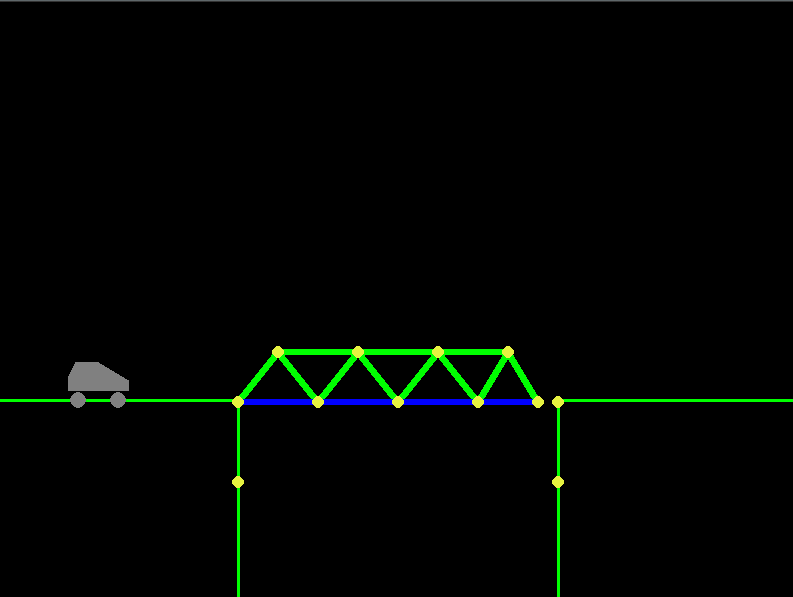
\includegraphics[width=\linewidth]{img/almost_good_bridge.png}
    \end{minipage}\hfill
    \begin{minipage}{0.49\textwidth}
        \centering
        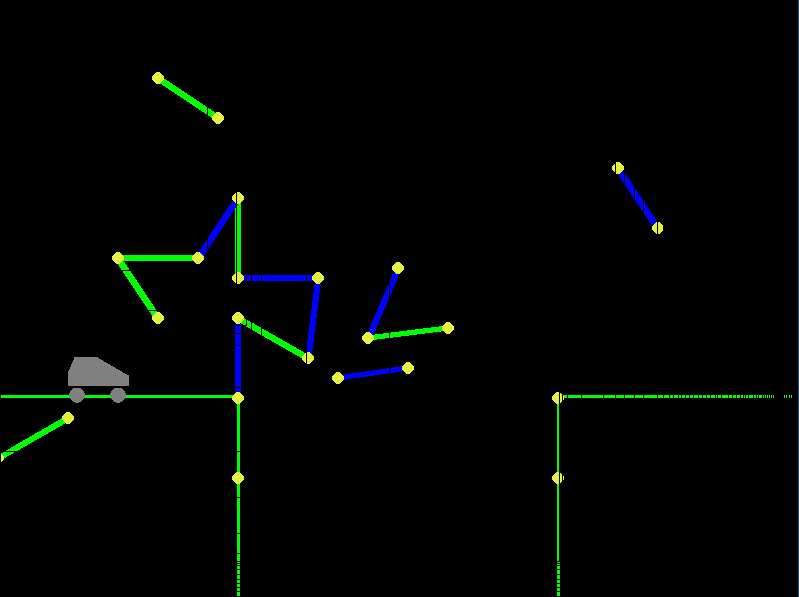
\includegraphics[width=\linewidth]{img/bad_bridge.png}
    \end{minipage}
    \caption{Dva mosty se stejnou fitness, ale rozdílných kvalit}
    \label{impl-fig:6}
\end{figure}

Navrhli jsem proto několik různých penalizací, které můžeme do fitness zapojit.

\begin{itemize}
    \item Penalizace za umisťování materiálů, který se nespojí s další materíálem. Lépe propojený most by měl mít lepší stabilitu
    \item Penalizace za všechny kotvy, které jedinec nepoužil. V praxi vzdálenosti každého kliknutí ke všem nepoužitým kotvám. Most který používá více kotev by měl být stabilnější
    \item Penalizace za předčasně ukončenou simulaci. Simulace se předčasně ukončí pokud vozidlo spadne, nebo pokud se dlouho nepohybuje.
\end{itemize}

Fitness pak bude odpovídat $f(g) = (-d_{min}(g) + \alpha \cdot mat + \beta \cdot anch + \gamma \cdot term, -cost(g))$, kde $\alpha, \beta, \gamma \in \R$ a $mat, anch, term$ jsou penalizace za nespojený materiál, nevyužité kontvy a předčasné ukončení.

Použijeme stejnou selekci a mutaci a reprezantaci jedince jako v předchozím návrhu.

\subsection{Měnící se fitness}

V rámci našeho přístupu jsme narazili na specifický problém spojený se stabilitou mostu. Spočívá v tom, že dokud není most zcela dokončen, nedosahuje potřebné stability, které je potřeba pro přejetí vozidlem. Abychom se s tímto omezením vypořádali, rozhodli jsme se pro zjednodušení problému a využití technik navrhnutých (citace IGA). Na začátku experimentu proto začínáme s břehy blíže umístěnými k sobě a jakmile dosáhneme dostatečně nízké průměrné fitness v celé populaci, vzdálenost postupně zvětšujeme, dokud nedosáhneme vzdálenosti definové úrovní. 

Použijeme stejnou selekci, mutaci a reprezantaci jedince jako v předchozím návrhu.

\subsection{Grafové kódování}

V této části bychom chtěli představit odlišný způsob, jak kódovat jednotlivce. Naše dosavadní kódovaní značně trpí tím, že je nepravděpodobné aby, se v jednom bodě spojilo více, než dva kusy materiálu. Tento problém se pokusíme vyřešit tím, že jedince budeme kódovat jako graf, tedy pomocí vrchlů a hran. To v praxi znamená, že gen jedince se skládá z množiny vrcholů $V$, množiny hran $E \subseteq V \times V$, funkce $\sigma_v : V \rightarrow \R^2$ která je projekcí $V$ do roviny a $\sigma_e : E \rightarrow T$. Naše navržené genetické operátory vypadají následovně.

\begin{itemize}
    \item \textbf{inicializace}: Do $V$ přidáme všechny kotvy z úrovně. Náhodně vybereme materiál $t \in T$, vrchol $v_1 \in V$, úhel $\varphi$ a délku $0 < l < l_{max}$. Vytvoříme nový vrchol $v_2$ a vložíme jej do $V$. Upravíme $\sigma_v$ tak, že $v_2$ se promítne na bod ve zvdálenosti $l$ a pod úhlem $\varphi$ od $\sigma_v(v_1)$. Vytvoříme novou hranu $(v_1, v_2)$ a přidáme jí do $E$ a zárověn upravíme $\sigma_e$ tak, že $\sigma_e((v_1, v_2)) = t$. Opakujeme dokud nevytvoříme $n$ nových vrcholů. Následně náhodně volíme dva vrcholy $v_1, v_2 \in V$. Pokud $||\sigma_v(v_1) - \sigma_v(v_2)|| < l_{max}$ vytvoříme novou hranu $(v_1, v_2)$ a přidáme do $E$. Upravíme $\sigma_e((v_1, v_2)) = t$ pro náhodně zvolené $t \in T$. Opakujeme $2n$-krát.
    \item \textbf{mutace}: Budeme rozlišovat mutaci pro vrcholy a mutaci pro hrany. Mutace pro vrcholy upraví $\sigma_v$ tak, že projekci vrcholu $v \in V$ přemístí na náhodně zvolený bod z $\{ x \in \R^2 | \forall v_2 \in Adj(v_1), ||x - \sigma_v(v_2)|| < l_{max}\}$ kde $Adj(v_1) = \{v \in V | (v_1, v) \in E\}$. Jinými slovy náhodně posumeme vrchol $v$ tak, aby nebyl příliš daleko od žádného vrcholu s nímž byl $v$ spojen hranou. Mutace pro hrany může hranu přidat, odebrat jí nebo změnit $\sigma_e$ náhodné hrany na jiný typ materiálu.
    \item \textbf{křížení}: Dva jedince můžeme skřížit následovně. Nechť $V_1, E_1$ je množina všech vrhcolů a hran prvního z rodičů a $V_2, E_2$ druhého. Nechť $\sigma_{v_p}$ je spojení $\sigma_v$ funkcí obou rodičů a $\sigma_{e_p}$ spojení $\sigma_e$ funkcí obou rodičů. Zvolíme náhodně hranici $min\{\sigma_{v_p}(v)_x | v \in V_1 \cup V_2\} < p_x < max\{\sigma_{v_p}(v)_x | v \in V_1 \cup V_2\}$. Nechť $L = \{ v | v \in V_1, \sigma_{v_p}(v)_1 < p_x\}$ a $R = \{ v | v \in V_2, \sigma_{v_p}(v)_1 > p_x\}$. Vrcholy genu potomka pak budou z $V_p = R + L$ a hrany $E_p = (E_1 + E_2) \cap V_p \times V_p$, kterým navíc přidáme všechny $(v_1, v_2), v_1 \in R, v_2 \in L, ||\sigma_{v_p}(v_1) - \sigma_{v_p}(v_2)|| < l_{max}$ s pravděpodobností $\alpha$. $\sigma_v$ potomka bude $sigma_{v_p}$ a stejně tak pro $\sigma_e$.
\end{itemize}

Jako selekci použijeme turnajovou selekci.

\subsection{Lepší inicializace}

Do našeho algoritmu múžeme ještě zahrnout jednu z nejsilnějších techni pro evoluční algoritmy a to použití \textit{domain-specific} znalostí (citace na domain specific). I když ještě nevim, jak bude optimální most vypadat, dokážeme obecným způsobem navrhnout most, který sice nebude optimální, ale bude lepší, než náhodně umístěný materiál. Z tohoto důvodu jsme implementovali postup podobný tomu, který navrhly (citace mosty). Tento postup se skládá ze tří kroků.

\begin{enumerate}
    \item \textbf{Vytvoření vozovky}: Nejprve pro vozidlo vytvoříme vozovku a to tím způsobem, spojíme levý a pravý břeh vozovkami a náhodné délce.
    \item \textbf{Vytvoření opor}: Následně pro každou ještě nevyužitou kotvu vyberem jeden spojový kloub z předchozího kroku a spojíme je dřevěnými díly o náhodné délce.
    \item \textbf{Zpevnění}: Nakonec pro každý přidaný materiál vytvoříme náhodně vybereme nový bod tak, abyhcom jej mohli spojit jedním dílem dřeva se začátkem a koncem tohoto materiálu a navíc bod spojíme se všemi ostatními bodu v blízkém okolí s pravděpodobností $\omega$.
\end{enumerate}

Vizualizaci těchto tří kroků můžme vidět na obrázku \ref{impl-fig:7}

\begin{figure}[ht]
    \centering
    \begin{minipage}{0.32\textwidth}
        \centering
        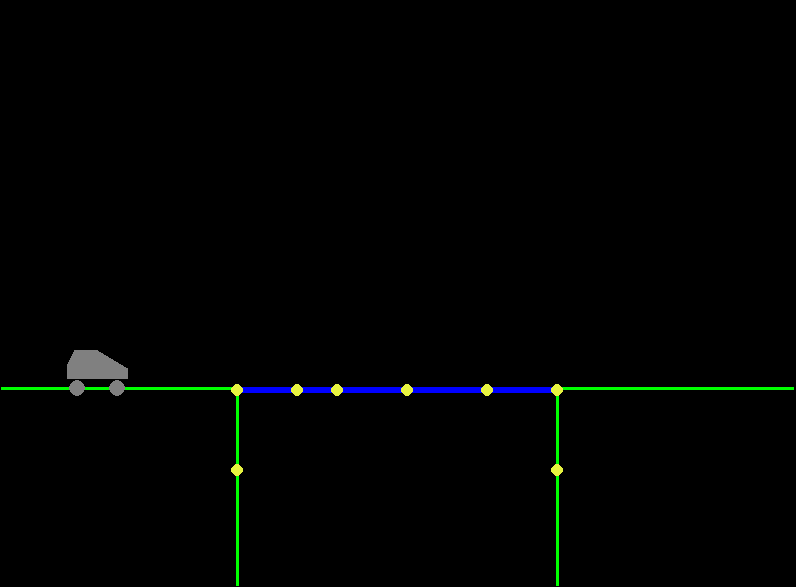
\includegraphics[width=\linewidth]{img/better_init1.png}
    \end{minipage}\hfill
    \begin{minipage}{0.32\textwidth}
        \centering
        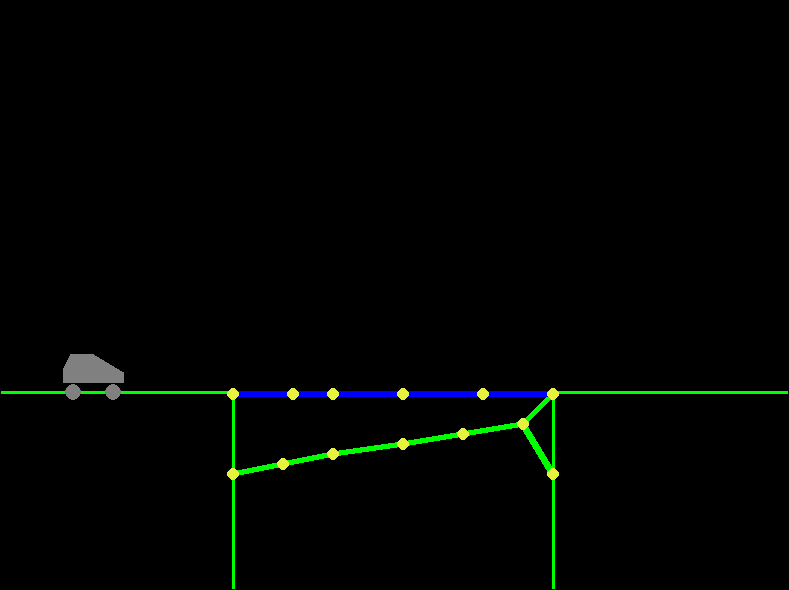
\includegraphics[width=\linewidth]{img/better_init2.png}
    \end{minipage}
    \begin{minipage}{0.32\textwidth}
        \centering
        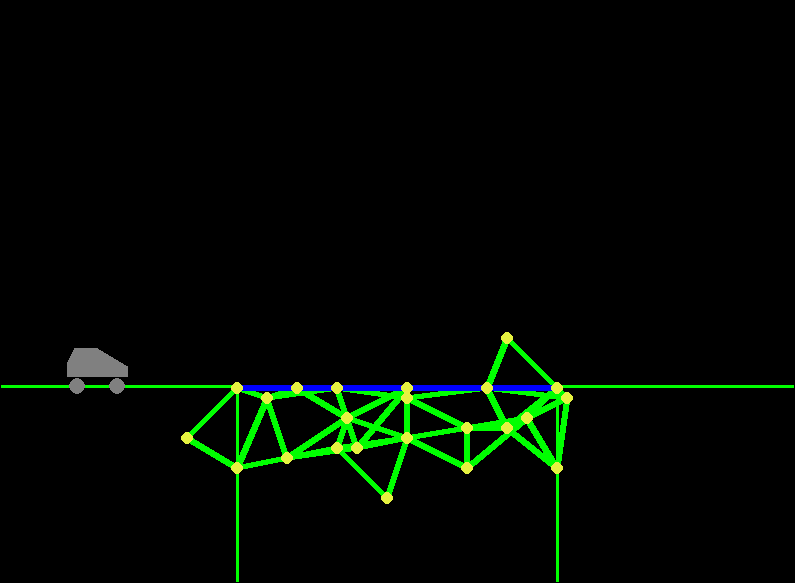
\includegraphics[width=\linewidth]{img/better_init3.png}
    \end{minipage}
    \caption{Výtváření jedince pomocí lepší inicializace. Krok \textbf{Vytvoření vozovky} vlevo, krok \textbf{Vytoření opor} uprostřed a krok \textbf{Zpevění} s $\omega = 1$ vpravo}
    \label{impl-fig:7}
\end{figure}

Použijeme selekci, křížení a mutaci z přechozího návrhu.
